\documentclass[10pt]{article}
\usepackage[margin=3cm]{geometry}
\usepackage{graphicx}
\usepackage{enumerate}
\usepackage[utf8]{inputenc}
\title{\bfseries\Huge 	Franco P. Bonafé}
\author{}
\date{}
\begin{document}
\hrule
\vspace{.25cm}
\begin{minipage}{0.65\textwidth}
\begingroup
\let\center\flushleft
\let\endcenter\endflushleft
\raggedleft{\maketitle}
\endgroup
\end{minipage}
\begin{minipage}{0.3\textwidth}
\flushright{
  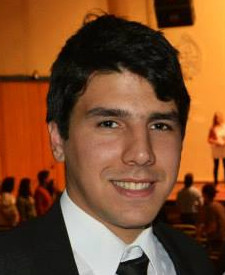
\includegraphics[width=3.0cm]{foto-franco.jpg}
}
\end{minipage}
\vspace{.25cm}
\hrule

\section{Información Personal}
\begin{itemize}
 \item {\bf Nombre completo:} Franco Paúl Bonafé
% \begin{tabular}{@{\hspace{18ex}}p{42em}}
% C\'ordoba, Argentina
% \end{tabular}
\item {\bf Fecha y lugar de Nacimiento:} 18 de Julio de 1990 - Córdoba, Argentina
\item {\bf DNI:} 36125009
 \item {\bf Domicilio particular:} Av. Valparaíso 2733, 5016, C\'ordoba
 \item {\bf Teléfono móvil:} 0351 15 547 2791
 \item {\bf Domicilio laboral:}  Dpto. de Matamática y Física, Facultad de Ciencias Químicas, UNC \\
 Instituto de Investigaciones en Fisicoquímica de Córdoba (INFIQC): CONICET, UNC \\
 Haya de la Torre esq. Medina Allende.
 Ciudad Universitaria, 5000, Córdoba
\item {\bf Teléfono laboral:} 0351 5353 853 Int. 55190
\item {\bf e-mail:} \texttt{fbonafe@fcq.unc.edu.ar} 
\item {\bf e-mail alternativo:} \texttt{francobonafe@gmail.com}
\end{itemize}

\section{Formación académica}
{\bf Títulos:}
\begin{itemize}
\item {\bf Licenciado en Química, Orientación: Fisicoquímica} (2009-2014) \\
Facultad de Ciencias Químicas, Universidad Nacional de Córdoba. \\
Promedio general (con aplazos): 9.82/10.
\item {\bf Bachiller Técnico en Producción de Bienes y Servicios,  \\ Orientación: Alimentación} (2003-2008) \\
Instituto Secundario Dr. Manuel Lucero (C\'ordoba). \\
Promedio general: 9.64/10.
\end{itemize}
{\bf En curso:}
\begin{itemize}
\item {\bf Estudiante de la carrera de Doctorado en Ciencias Químicas} \\
Facultad de Ciencias Químicas, Universidad Nacional de Córdoba. \\
Trabajo de tesis: ``Relajación de excitaciones electrónicas en sistemas nanoscópicos''. \\
Director: Cristián G. Sánchez. \\
Beca de  posgrado de CONICET. 
Unidad Académica: INFIQC (CONICET - UNC). 
\end{itemize}

\section{Docencia e investigación}

\subsection{Actividades docentes}
{\bf Cargos como auxiliar docente}
\begin{itemize}
 \item {\bf Profesor Asistente}, dedicación simple, interino - Res. 320/15 H.C.D. \\ Dpto. de Matemática y Física, Fac. Cs. Químicas, UNC. 01/10/2014-actualidad.
 \item {\bf Profesor Ayudante B}, dedicación simple, {\bf por concurso} - Res. 154/15 H.C.D. \\ Dpto. de Matemática y Física, Fac. Cs. Químicas, UNC. 01/04/2004-actualidad. En licencia.
 \item { Profesor Asistente}, dedicación simple, interino - Res. 967/14 H.C.D. \\ Dpto. de Matemática y Física, Fac. Cs. Químicas, UNC. 01/10/2014-31/03/2015.
\end{itemize}
{\bf Cargos como alumno}
\begin{itemize}
 \item { Ayudante alumno Cat. A} - Res. 700/13 H.C.D. \\ Dpto. de Matemática y Física, Fac. Cs. Químicas, UNC. 01/09/2013-31/08/2014.
 \item { Ayudante alumno del Ciclo de Nivelación 2013} - Res. 1076/12 H.C.D. \\ Fac. Cs. Químicas, UNC. 01-04/2013.
 \item { Ayudante alumno Cat. A} - Res. 735/12 H.C.D. \\ Dpto. de Fisicoquímica, Fac. Cs. Químicas, UNC. 01/09/2012-31/08/2013.
 \item { Ayudante alumno Cat. B} - Res. 747/11 H.C.D \\ Dpto. de Fisicoquímica, Fac. Cs. Químicas, UNC. 01/09/2011-31/08/2012.
 \item { Ayudante ad-honorem} - Res. 1/11, 807/11 H.C.D. \\ Dptos. de Matemática y Física y Fisicoquímica, Fac. Cs. Químicas, UNC. 09/2010-05/2011.
\end{itemize}
{\bf Labor en docencia de grado}
\begin{itemize}
 \item 2015: Matemática III (jefe de trabajos prácticos).
 \item 2014: Matemática I (ayudante alumno), Matemática II (auxiliar)
 \item 2013: Ciclo de Nivelación, Laboratorio I (ayudante alumno), 2do cuatrimestre de licencia por estadía en el exterior.
 \item 2012: Laboratorio III, Química Analitica General (ayudante alumno)
 \item 2011: Matemática I (ad-honorem), Química Analítica General (ayudante alumno)
 \item 2010: Laboratorio II (ad-honorem)
\end{itemize}
{\bf Formación docente}
 \begin{itemize}
  \item Asistente a la jornada ``Educando al Cerebro'': estrategias neuroeducativas aplicadas a los diferentes niveles educativos. Aprobado por CONICET y VocAr. Ciudad Universitaria, Córdoba, 9/08/2014.
 \end{itemize}

\subsection{Publicaciones}
\begin{enumerate}
\item{\it ``Ultra-small rhenium clusters  supported on graphene''}, O. Miramontes, F.P. Bonafé, U. Santiago, E. Larios Rodríguez, J.J. Velázquez-Salazar, M. Mariscal, M. Jose-Yacamán. Phys. Chem. Chem. Phys. (2015) {\bf 17} 7898.
\item{\it ``A theoretical study of the optical properties of nanostructured TiO$_2$''}, V.C. Fuertes, C.F.A. Negre, M.B. Oviedo, F.P. Bonaf\'e, F.Y. Oliva and C.G. S\'anchez. J. Phys.: Cond. Matter (2013) {\bf 25} 115304.
\end{enumerate}

% \subsection{Publicaciones enviadas}
% \begin{enumerate}
%  \item{\it ``Photovoltaics from Automated, Ultra-Sonic Spray-Deposited Cu(In,Ga)Se$_2$ Nanocrystal Films''}, T.B. Harvey, F. Bonafé, T. Updegrave, V. Reddy, C. Thomas, S. C. Kamarajugadda, C.J. Stolle, D. Pernik, J. Du, B.A. Korgel. 2014. (en proceso de escritura) 
% \end{enumerate}

\subsection{Participación en reuniones científicas}
{\bf Internacionales}
\begin{enumerate}
 \item{\it ``Study of the nucleation of Pd nanoparticles on graphene''}. F. P. Bonafé, G. J. Soldano, M. M. Mariscal.
 XXII International Materials Research Congress (IMRC). Cancún, México. Agosto 2013.
 \item{\it ``Selenization of Automated, Ultra-Sonic Spray-Deposited Cu(In,Ga)Se$_2$ Nanocrystal Films for Photovoltaics''}. T. B. Harvey, F. P. Bonafé, T. Updegrave, C. Thomas, S. Kamarajugadda, C. J. Stolle, D. Pernik, J. Du and B. A. Korgel. AIChE Annual Meeting. Atlanta, Georgia, Estados Unidos. Noviembre 2014.
\end{enumerate}
{\bf Nacionales}
\begin{enumerate}
 \item{\it ``Nanomotor modelo impulsado por luz polarizada''}. Presentación oral. F. P. Bonafé, C. G. Sánchez.
 XIX Congreso Argentino de Fisicoquímica y Química Inorgánica. Buenos Aires, Argentina. Abril 2015.
 \item{\it ``TiO$_2$ como material de ánodo para baterías de ion-litio: un estudio computacional''}. F. P. Bonafé, F. Y. Oliva, G. L. Luque.
 5to. Congreso nacional - 4to. Congreso iberoamericano ``Hidrógeno y fuentes sustentables de energía'' (HYFUSEN). Córdoba, Argentina. Junio 2013.
%  \item{Segundo Encuentro Nacional de Computación de Alto Rendimiento para Aplicaciones Científicas}.  \\
%  Asistente. Facultad de Matemática, Astronomía y Física, UNC. Córdoba, Argentina. Mayo 2013.	
 \item {\it ``Estudio por cálculos DFT and DFT+U de la interacción de litio con diferentes polimorfos de TiO$_2$''}. F. P. Bonafé, F. Y. Oliva, G. L. Luque. 
 XVIII Congreso Argentino de Fisicoquímica y Química Inorgánica. Rosario, Argentina. Abril 2013.
 \item {\it ``Estudio de los parámetros estructurales que influyen en la reactividad superficial de nanopartículas de TiO$_2$''}. F. P. Bonafé, V. C. Fuertes, C. F. A. Negre, M. B. Oviedo, F. Y. Oliva, C. G. Sánchez.
 XVIII Congreso Argentino de Fisicoquímica y Química Inorgánica. Rosario, Argentina. Abril 2013.
%  \item {Encuentro Nanoc\'ordoba 2012}. Asistente. Villa Carlos Paz, Córdoba, Argentina. Octubre 2012.
%  \item {Simposio internacional en Buenos Aires: ``Desafíos en las baterías recargables de litio oxígeno''}. Asistente.
%  INQUIMAE - Facultad de Ciencias Exactas y Naturales, Universidad de Buenos Aires. Buenos Aires, Argentina. Septiembre 2012.
 \item {\it ``Efecto de la serie de Hofmeister sobre las propiedades ácido-base de la albúmina sérica humana: estudio experimental y modelo teórico''}. F. P. Bonafé, O. R. Cámara, F. Y. Oliva.
 XVII Congreso Argentino de Fisicoquímica y Química Inorgánica. Córdoba, Argentina. Mayo 2011.
\end{enumerate}

  \subsection{Becas obtenidas}
  \begin{itemize}
   \item {\bf Beca interna doctoral} del Consejo Nacional de Investigaciones Científicas y Técnicas por el término de 60 meses a partir del 1 de abril de 2014. Director: Dr. Cristián Sánchez. Puntaje: 96,30/100. 17/12/2013 - Res. D. 4830/2013 CONICET.
   \item Beca de movilidad estudiantil {\bf Programa Cuarto Centenario}. Exención de matrícula y ayuda económica. Prosecretaría de Relaciones Internacionales, UNC. 2do cuatrimestre de 2013 cursado en la {\bf Universidad de Texas en Austin}, Estados Unidos.
   \item Becario expositor en ``{\bf Cuatrociencia}: Muestra de Ciencia, Arte y Tecnología de la UNC''. 03/2103-04/2013 - Res. Rectoral 483/13.
   \item Beca de estímulo a las vocaciones científicas del {\bf Consejo Interuniversitario Nacional} (CIN). 
  %  Tema: Estudios experimentales y teóricos de incorporación de cationes de metales alcalinos 	en TiO$_2$. 
   Directoras: Dra. Fabiana Oliva, Dra. Guillermina Luque. Puntaje: 98.80/100. 09/2012-08/2013 - Res. Rectoral 2724/12.
   \item Beca de estímulo a las vocaciones científicas del {\bf Consejo Interuniversitario Nacional} (CIN). 
  %  Efecto de la naturaleza del electrolito en el desarrollo de carga de proteínas. Su aplicación en el proceso de adsorción sobre superficies de óxidos metálicos. 
   Directora: Dra. Fabiana Oliva. Puntaje: 98.92/100. 09/2011-08/2012 - Res. Rectoral 2382/11.
  \end{itemize}

\subsection{Trabajos de investigación}
\begin{itemize}
 \item {Doctorado en Ciencias Químicas} (04/2014-actualidad) \\
 ``Relajación de excitaciones electrónicas en sistemas nanoscópicos''.
 INFIQC (CONICET - UNC). Departamento de Matemática y Física, Fac. Cs. Químicas, Universidad Nacional de Córdoba.
 \item {Practicanato de Licenciatura en Química, parte 2} (08/2013-12/2013) \\
 ``Copper indium gallium selenide (CIGS) photovoltaic devices made using selenization of nanocrystal thin films''. Director: Brian A. Korgel. Department of Chemical Engineering, The University of Texas at Austin. Estados Unidos.
 \item {Practicanato de Licenciatura en Química, parte 1} (03/2013-07/2013) \\
 ``Estudio teórico del mecanismo de nucleación de nanopartículas de Pd sobre grafeno con aplicaciones en sensores de hidrógeno''. Departamento de Matemática y Física, Fac. Cs. Químicas, Universidad Nacional de Córdoba.
 \item {Trabajo de investigación como alumno de grado (Beca del CIN)} (09/2012-08/2013) \\ 
 ``Estudios experimentales y teóricos de incorporación de cationes de metales alcalinos en óxido de titanio.'' Departamentos de Fisicoquímica y de Matemática y Física, Fac. Cs. Químicas, Universidad Nacional de Córdoba.
 \item {Trabajo de investigación como alumno de grado (Beca del CIN)} (09/2011-08/2012) \\ 
 ``Efecto de la naturaleza del electrolito en el desarrollo de carga de proteínas. Su aplicación en el proceso de adsorción sobre superficies de óxidos metálicos.'' Departamento de Fisicoquímica, Fac. Cs. Químicas, Universidad Nacional de Córdoba. 
\end{itemize}

\subsection{Cursos realizados}
 \begin{itemize}
  \item {\bf Curso de posgrado} de formación general: ``La problemática de las ciencias químicas en Argentina''. Fac. Cs. Químicas, Universidad Nacional de Córdoba. 08/2041-12/2014 (finalizado). Directoras: Dra. Marcela Longhi, Dra. Mariana Rojas. Calificación y certificación en trámite.
  \item {\bf Curso de posgrado}: ``Métodos mecanocuánticos basados en la DFT. Aplicaciones a sistemas nanoestructurados''. Fac. Cs. Químicas, Universidad Nacional de Córdoba. 08/2014. Director: Ezequiel Leiva. Calificación: 10 (diez).
  \item {Microsoft Azure for Research Training.} Córdoba, Argentina, agosto 2014. 
  \item {\bf 3ra Escuela Argentina de GPGPU Computing para aplicaciones científicas.} San Carlos de Bariloche, Argentina, mayo 2014. Examen aprobado.
   \begin{itemize}
   \item {\it CUDA básico}. Pablo Ezzatti, Universidad de la República, Uruguay. 
   \item {\it A crash course on Multi-GPU computing}. Massimo Bernaschi, CUDA fellow, Universidad ``La Sapienza'', Italia.
   \item {\it PyOpenCL: OpenCL in Python}. Andreas Klöckner, UIUC, EEUU.
   \item {\it Medical image processing}. Anders Eklund, Virginia Tech, EEUU.
   \item {\it Física computacional con GPUSs}. Eduardo Bringa, UNCuyo, Argentina.
   \end{itemize}
  \item {\bf Clases tomadas en la Universidad de Texas en Austin, fall 2013}. Austin, Texas, Estados Unidos.
   \begin{itemize}
    \item {\it Quantum Mechanics I}. Steven Weinberg. Curso de posgrado. Calificación: A.
    \item {\it Quantum Physics II}. Daniel Heinzen. Curso de grado. Calificación: A.
    \item {\it Thermodynamics and Statistical Mechanics}. Elaine Li. Curso de grado. Calificación: A.
   \end{itemize}
  \item {\bf Cursos dictados en el Congreso HYFUSEN 2013}
  \begin{itemize}
   \item {\it Estado del arte de las baterías de litio. Dr. J. Thomas, INIFTA.}
   \item {\it Seguridad en la producción y utilización del hidrógeno. Ing. J. L. Aprea, CNEA.}
  \end{itemize} 
  \item {Curso de Electrónica Básica}. Academia Santo Domingo. 2008.
 \end{itemize}

\section{Actividades institucionales, de extensión y articulación}
\begin{itemize}
 \item Director del proyecto de articulación con escuelas secundarias {\bf ``Pensando la Ciencia''}, aprobado por Res. 374/15 H.C.D. Monto otorgado: \$2000.
 \item Coordinador de la actividad de articulación {\bf ``Semana de la Ciencia 2015''} por el Departamento de Matemática y Física, Facultad de Ciencias Químicas.
 \item Miembro titular de la {\bf Comisión de Articulación} con Escuelas Secundarias de la Facultad de Ciencias Químicas.  11/2014-actualidad - Res. 1040/14 H.C.D.
 \item Expositor en la {\bf ``Semana de la Ciencia 2014''} de la Facultad de Ciencias Químicas, en el módulo: ``Simuladores al rescate''. 08/2014 - Res. 923/14 H.C.D. 
 \item { Miembro del comité evaluador de carrera docente}, Facultad de Ciencias Químicas. Observador estudiantil. 06/2013 - Res. 129/13 H.C.D. 
 \item  Becario expositor en Muestra de Ciencia, Arte y Tecnología {\bf ``Cuatrociencia''}. Stand: ``Revolución energética para un futuro sustentable''. 03/2013-04/2013 - Res. Rectoral 483/13 
 \item Participación en calidad de organizador del stand ``Revolución energética para un futuro sustentable'' en la muestra {\bf Cuatrociencia}. Fabricación de un aparato de electrólisis y póster - Res. 497/13 H.C.D.
%  \item { Asistente en las III Jornadas de Articulación de la Fac. Cs. Químicas}. 30/11/2012. 
 \item Orador en muestra de carreras {\bf ``La UNC te espera''}, Facultad de Ciencias Químicas. Experimentos demostrativos. 09/2012 - Res. 886/12 H.C.D.
 \item A cargo del entrenamiento de los alumnos del Instituto Dr. Manuel Lucero para la Olimpíada Argentina de Química. 2008-2013.
%  \item { Orador en programa de articulación ``Química Joven 2012''}. Charlas en colegios secundarios para promoción del estudio de la ciencia. 06/2012-08/2012 - Res. Decanal 675/12
 \end{itemize}
 
 \section{Emprendedorismo y transferencia tecnológica}
 \begin{itemize}
  \item Emprendedor resposable del proyecto ``Óptica in Sílico'' seleccionado para ingresar el sistema de incubación de la {\bf Incubadora de Empresas} del Parque Científico Tecnológico de la UNC - Res. SECyT UNC 390/14.
  \item ``Emprededor E+E'' otorgado por la Fundación Empresarial para Emprendedores. Aprobación del seminario de planes de negocios. 11/2011.
  \item Primer puesto en concurso de planes de negocios del programa Emprendedores Tecnológicos 2010, organizado por Junior Achievement, Motorola y Banco Galicia. Buenos Aires, 24/11/2010.
%   \item Seminario Emprendedores Tecnológicos, organizado por Junior Achievement, Motorola y Banco Galicia. Córdoba, 8/05/2010.
 \end{itemize}

 \section{Conocimiento de idiomas}
\begin{itemize}
\item{\bf Inglés.} Nivel B2. Diplomas:
\begin{itemize}
\item {\bf First Certificate in English} (2007) \\
University of Cambridge ESOL Examinations\\
Grade: A
\item {\bf Preliminary English Test} (2006) \\
University of Cambridge ESOL Examinations \\
Grade: Pass with Merit
\end{itemize}
\end{itemize}
 
\section{Premios}
\begin{itemize}
\item Medalla al Mejor Promedio de la Universidad Nacional de Córdoba Promoción 2013.
\item {\bf Premio Universidad 2013}: Diploma con ``Mención de Honor'' - Res. Rectoral 1243/14.
\item {Premio a la excelencia académica}, Banco Roela, año 2008. Otorgado al mejor alumno graduado de la escuela secundaria.
\item {Medalla de mérito académico}, Instituto Secundario Dr. Manuel Lucero, año 2008. Otorgado al mejor alumno del último año de la escuela secundaria.
\end{itemize}

\section{Otros reconocimientos}
\begin{itemize}
\item Abanderado de la Facultad de Ciencias Químicas, Universidad Nacional de Córdoba, año 2013 - Res. 726/13 H.C.D. 
% Mérito al mejor promedio del último año de las carreras de la Facultad.
\item {Primer escolta de la bandera nacional de la Universidad Nacional de Córdoba, año 2013 - Res. Rectoral 1439/13}.
% Merito al segundo mejor promedio de la Universidad.
 \item {Segundo escolta de la bandera nacional de la Facultad de Ciencias Químicas, Universidad Nacional de Córdoba, año 2012 - Res. 688/12 H.C.D.}
%  Mérito al mejor promedio del penúltimo año de las carreras de la Facultad.
 \item {Preselección para la Olimpíada Internacional de Química 2009}. Entrenamiento teórico práctico de 2 meses en la FCEN, UBA, como preparación para la IChO 2009 (Reino Unido).
 \item {Olimpíada Argentina de Química}, Universidad de Buenos Aires. Medalla de oro en nivel 1 (2007) y nivel 2 (2008). Mejor examen regional (2007 y 2008).
 \item {Feria de Ciencia y Tecnología}, Agencia Córdoba Ciencia y Ministerio de Ciencia y Tecnología.
%  Proyecto: {\it ``El poder del agua: estudio de los parámetros electroquímicos y termodinámicos que intervienen en el rendimiento de los procesos
% electrolíticos para la optimización de la electrólisis del agua''}. 
Diploma de mención especial (2006). 2do. lugar en etapa provincial (2007). Participación en instancia
nacional, Ciudad Autónoma de Buenos Aires (2007).
\item {Olimpíada de Matemática Argentina.} Diploma de mención especial en instancia provincial (2008). Promoción a la instancia nacional (2007).
\end{itemize}

\end{document}